
\documentclass[letterpaper,hide notes,xcolor={table,svgnames},pdftex,10pt]{beamer}
\def\showexamples{t}


%\usepackage[svgnames]{xcolor}

%% Demo talk
%\documentclass[letterpaper,notes=show]{beamer}

\usecolortheme{crane}
\setbeamertemplate{navigation symbols}{}

\usetheme{MyPittsburgh}
%\usetheme{Frankfurt}

%\usepackage{tipa}

\usepackage{hyperref}
\usepackage{graphicx,xspace}
\usepackage[normalem]{ulem}
\usepackage{multicol}
\usepackage{amsmath,amssymb,amsthm,graphicx,xspace}
\newcommand\SF[1]{$\bigstar$\footnote{SF: #1}}

\usepackage[default]{sourcesanspro}
\usepackage[T1]{fontenc}

\newcounter{tmpnumSlide}
\newcounter{tmpnumNote}

% old question code
%\newcommand\question[1]{{$\bigstar$ \small \onlySlide{2}{#1}}}
% \newcommand\nquestion[1]{\ifdefined \presentationonly \textcircled{?} \fi \note{\par{\Large \textbf{?}} #1}}
% \newcommand\nanswer[1]{\note{\par{\Large \textbf{A}} #1}}


 \newcommand\mnote[1]{%
   \addtocounter{tmpnumSlide}{1}
   \ifdefined\showcues {~\tiny\fbox{\arabic{tmpnumSlide}}}\fi
   \note{\setlength{\parskip}{1ex}\addtocounter{tmpnumNote}{1}\textbf{\Large \arabic{tmpnumNote}:} {#1\par}}}

\newcommand\mmnote[1]{\note{\setlength{\parskip}{1ex}#1\par}}

%\newcommand\mnote[2][]{\ifdefined\handoutwithnotes {~\tiny\fbox{#1}}\fi
% \note{\setlength{\parskip}{1ex}\textbf{\Large #1:} #2\par}}

%\newcommand\mnote[2][]{{\tiny\fbox{#1}} \note{\setlength{\parskip}{1ex}\textbf{\Large #1:} #2\par}}

\newcommand\mquestion[2]{{~\color{red}\fbox{?}}\note{\setlength{\parskip}{1ex}\par{\Large \textbf{?}} #1} \note{\setlength{\parskip}{1ex}\par{\Large \textbf{A}} #2\par}\ifdefined \presentationonly \pause \fi}

\newcommand\blackboard[1]{%
\ifdefined   \showblackboard
  {#1}
  \else {\begin{center} \fbox{\colorbox{blue!30}{%
         \begin{minipage}{.95\linewidth}%
           \hspace{\stretch{1}} Some space intentionally left blank; done at the blackboard.%
         \end{minipage}}}\end{center}}%
         \fi%
}



%\newcommand\q{\tikz \node[thick,color=black,shape=circle]{?};}
%\newcommand\q{\ifdefined \presentationonly \textcircled{?} \fi}

\usepackage{listings}
\lstset{%
  keywordstyle=\bfseries,
  aboveskip=15pt,
  belowskip=15pt,
  captionpos=b,
  identifierstyle=\ttfamily,
  escapeinside={(*@}{@*)},
  stringstyle=\ttfamiliy,
  frame=lines,
  numbers=left, basicstyle=\scriptsize, numberstyle=\tiny, stepnumber=0, numbersep=2pt}

\usepackage{siunitx}
\newcommand\sius[1]{\num[group-separator = {,}]{#1}\si{\micro\second}}
\newcommand\sims[1]{\num[group-separator = {,}]{#1}\si{\milli\second}}
\newcommand\sins[1]{\num[group-separator = {,}]{#1}\si{\nano\second}}
\sisetup{group-separator = {,}, group-digits = true}

%% -------------------- tikz --------------------
\usepackage{tikz}
\usetikzlibrary{positioning}
\usetikzlibrary{arrows,backgrounds,automata,decorations.shapes,decorations.pathmorphing,decorations.markings,decorations.text}

\tikzstyle{place}=[circle,draw=blue!50,fill=blue!20,thick, inner sep=0pt,minimum size=6mm]
\tikzstyle{transition}=[rectangle,draw=black!50,fill=black!20,thick, inner sep=0pt,minimum size=4mm]

\tikzstyle{block}=[rectangle,draw=black, thick, inner sep=5pt]
\tikzstyle{bullet}=[circle,draw=black, fill=black, thin, inner sep=2pt]

\tikzstyle{pre}=[<-,shorten <=1pt,>=stealth',semithick]
\tikzstyle{post}=[->,shorten >=1pt,>=stealth',semithick]
\tikzstyle{bi}=[<->,shorten >=1pt,shorten <=1pt, >=stealth',semithick]

\tikzstyle{mut}=[-,>=stealth',semithick]

\tikzstyle{treereset}=[dashed,->, shorten >=1pt,>=stealth',thin]

\usepackage{ifmtarg}
\usepackage{xifthen}
\makeatletter
% new counter to now which frame it is within the sequence
\newcounter{multiframecounter}
% initialize buffer for previously used frame title
\gdef\lastframetitle{\textit{undefined}}
% new environment for a multi-frame
\newenvironment{multiframe}[1][]{%
\ifthenelse{\isempty{#1}}{%
% if no frame title was set via optional parameter,
% only increase sequence counter by 1
\addtocounter{multiframecounter}{1}%
}{%
% new frame title has been provided, thus
% reset sequence counter to 1 and buffer frame title for later use
\setcounter{multiframecounter}{1}%
\gdef\lastframetitle{#1}%
}%
% start conventional frame environment and
% automatically set frame title followed by sequence counter
\begin{frame}%
\frametitle{\lastframetitle~{\normalfont(\arabic{multiframecounter})}}%
}{%
\end{frame}%
}
\makeatother

\makeatletter
\newdimen\tu@tmpa%
\newdimen\ydiffl%
\newdimen\xdiffl%
\newcommand\ydiff[2]{%
    \coordinate (tmpnamea) at (#1);%
    \coordinate (tmpnameb) at (#2);%
    \pgfextracty{\tu@tmpa}{\pgfpointanchor{tmpnamea}{center}}%
    \pgfextracty{\ydiffl}{\pgfpointanchor{tmpnameb}{center}}%
    \advance\ydiffl by -\tu@tmpa%
}
\newcommand\xdiff[2]{%
    \coordinate (tmpnamea) at (#1);%
    \coordinate (tmpnameb) at (#2);%
    \pgfextractx{\tu@tmpa}{\pgfpointanchor{tmpnamea}{center}}%
    \pgfextractx{\xdiffl}{\pgfpointanchor{tmpnameb}{center}}%
    \advance\xdiffl by -\tu@tmpa%
}
\makeatother
\newcommand{\copyrightbox}[3][r]{%
\begin{tikzpicture}%
\node[inner sep=0pt,minimum size=2em](ciimage){#2};
\usefont{OT1}{phv}{n}{n}\fontsize{4}{4}\selectfont
\ydiff{ciimage.south}{ciimage.north}
\xdiff{ciimage.west}{ciimage.east}
\ifthenelse{\equal{#1}{r}}{%
\node[inner sep=0pt,right=1ex of ciimage.south east,anchor=north west,rotate=90]%
{\raggedleft\color{black!50}\parbox{\the\ydiffl}{\raggedright{}#3}};%
}{%
\ifthenelse{\equal{#1}{l}}{%
\node[inner sep=0pt,right=1ex of ciimage.south west,anchor=south west,rotate=90]%
{\raggedleft\color{black!50}\parbox{\the\ydiffl}{\raggedright{}#3}};%
}{%
\node[inner sep=0pt,below=1ex of ciimage.south west,anchor=north west]%
{\raggedleft\color{black!50}\parbox{\the\xdiffl}{\raggedright{}#3}};%
}
}
\end{tikzpicture}
}


%% --------------------

%\usepackage[excludeor]{everyhook}
%\PushPreHook{par}{\setbox0=\lastbox\llap{MUH}}\box0}

%\vspace*{\stretch{1}

%\setbox0=\lastbox \llap{\textbullet\enskip}\box0}

\setlength{\parskip}{\fill}

\newcommand\noskips{\setlength{\parskip}{1ex}}
\newcommand\doskips{\setlength{\parskip}{\fill}}

\newcommand\xx{\par\vspace*{\stretch{1}}\par}
\newcommand\xxs{\par\vspace*{2ex}\par}
\newcommand\tuple[1]{\langle #1 \rangle}
\newcommand\code[1]{{\sf \footnotesize #1}}
\newcommand\ex[1]{\uline{Example:} \ifdefined \presentationonly \pause \fi
  \ifdefined\showexamples#1\xspace\else{\uline{\hspace*{2cm}}}\fi}

\newcommand\ceil[1]{\lceil #1 \rceil}


\AtBeginSection[]
{
   \begin{frame}
       \frametitle{Outline}
       \tableofcontents[currentsection]
   \end{frame}
}



\pgfdeclarelayer{edgelayer}
\pgfdeclarelayer{nodelayer}
\pgfsetlayers{edgelayer,nodelayer,main}

\tikzstyle{none}=[inner sep=0pt]
\tikzstyle{rn}=[circle,fill=Red,draw=Black,line width=0.8 pt]
\tikzstyle{gn}=[circle,fill=Lime,draw=Black,line width=0.8 pt]
\tikzstyle{yn}=[circle,fill=Yellow,draw=Black,line width=0.8 pt]
\tikzstyle{empty}=[circle,fill=White,draw=Black]
\tikzstyle{bw} = [rectangle, draw, fill=blue!20, 
    text width=4em, text centered, rounded corners, minimum height=2em]
    
    \newcommand{\CcNote}[1]{% longname
	This work is licensed under the \textit{Creative Commons #1 3.0 License}.%
}
\newcommand{\CcImageBy}[1]{%
	\includegraphics[scale=#1]{creative_commons/cc_by_30.pdf}%
}
\newcommand{\CcImageSa}[1]{%
	\includegraphics[scale=#1]{creative_commons/cc_sa_30.pdf}%
}
\newcommand{\CcImageNc}[1]{%
	\includegraphics[scale=#1]{creative_commons/cc_nc_30.pdf}%
}
\newcommand{\CcGroupBySa}[2]{% zoom, gap
	\CcImageBy{#1}\hspace*{#2}\CcImageNc{#1}\hspace*{#2}\CcImageSa{#1}%
}
\newcommand{\CcLongnameByNcSa}{Attribution-NonCommercial-ShareAlike}

\newenvironment{changemargin}[1]{% 
  \begin{list}{}{% 
    \setlength{\topsep}{0pt}% 
    \setlength{\leftmargin}{#1}% 
    \setlength{\rightmargin}{1em}
    \setlength{\listparindent}{\parindent}% 
    \setlength{\itemindent}{\parindent}% 
    \setlength{\parsep}{\parskip}% 
  }% 
  \item[]}{\end{list}} 




\title{Tutorial 4 --- Storage, B+ Trees}

\author{Richard Wong \\ \small \texttt{rk2wong@edu.uwaterloo.ca}}
\institute{Department of Electrical and Computer Engineering \\
  University of Waterloo}
\date{\today}


\begin{document}

\begin{frame}
  \titlepage

\end{frame}


\begin{frame}
\frametitle{Exercise 4-1}

Does the data in a heap file necessarily lie in a contiguous region in secondary memory (disk)?

\end{frame}


\begin{frame}
\frametitle{Exercise 4-1 Solution}

No, recall that a file is a logical abstraction.
The OS filesystem manages the blocks that make up our files.
These blocks can exist apart from one another in physical memory.

\end{frame}


\begin{frame}
\frametitle{Exercise 4-2}

Why would we use a B+ tree file instead of a sorted file to hold our database records?

\end{frame}


\begin{frame}
\frametitle{Exercise 4-2 Solution}

Suppose our database contains more data than fits in main memory.

How would you search the sorted file? The binary search algorithm requires us to know the midpoint of our sorted collection.

The B+ tree allows us to perform O(log n) lookups/insertions/deletions without a O(n) memory footprint.

The B+ tree also lets us narrow down lookup results by more than a factor of 2 with each iteration of the lookup algorithm.

\end{frame}


\begin{frame}
\frametitle{Exercise 4-3}

When might we want to use a hash file instead of a B+ tree file to hold our database records?

\end{frame}


\begin{frame}
\frametitle{Exercise 4-3 Solution}

The hash file grants us constant-time lookup by key, but not much else.

If we expect a significant portion of our queries to be lookups by key equality, this could be good (but comparisons, ordering, etc. will be sloooooow...)

\end{frame}


\begin{frame}
\frametitle{Exercise 4-4}

When would we prefer MRU over LRU as a database cache replacement algorithm?

\end{frame}


\begin{frame}
\frametitle{Exercise 4-4 Solution}

This depends on memory access patterns.

MRU is good under the assumption that blocks we have used recently are less likely to be accessed soon. This is typically true with database systems.

This is the opposite assumption that LRU makes (temporal locality). We might want to use LRU in a more generalized setting (OS memory management, where the OS doesn't know memory access patterns of applications).

\end{frame}


\begin{frame}
\frametitle{Exercise 4-5}

Why shouldn't we make lots of indices over our database tables?

\end{frame}


\begin{frame}
\frametitle{Exercise 4-5 Solution}

Each index on our table introduces a time overhead with each record update, insertion, and deletion, if we want to keep our indices up to date (which is likely, in our single-machine environment).

Indices also take up space. Ideally, all of our indices fit in main memory; otherwise, we pay the cost of disk swap.

In short, database writes become increasingly expensive with more indices.

\end{frame}


\begin{frame}
\frametitle{Exercise 4-6}

Insert the following keys into the B+ tree below with degree $d$=2:

\texttt{Adams}\\
\texttt{Lamport}

\begin{center}
  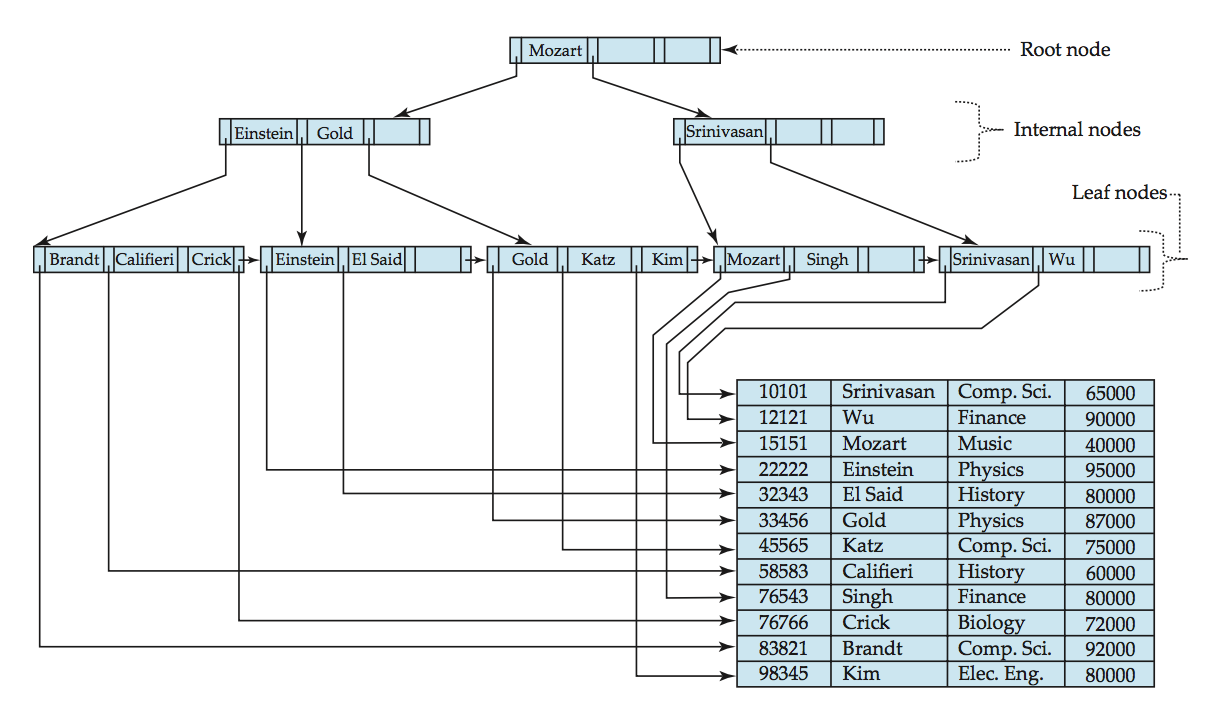
\includegraphics[width=0.9\textwidth]{images/b-tree-complete.png}
\end{center}

\end{frame}


\begin{frame}
\frametitle{Exercise 4-6 Solution (1/2)}

As an aside, we know the degree is 2 because the nodes/blocks have at most \\
4 = 2$d$ child pointers.

\texttt{insert(Adams)}

Follow the tree to find out where to insert Adams.

This ends up being left of Brandt/Califieri/Crick, but that block is full. (Conceptually) add it anyways.

Split the oversized block into Adams/Brandt and Califieri/Crick.

Promote Califieri (leftmost key of right split) as a key in the parent such that the parent becomes Califieri/Einstein/Gold.

\begin{center}
  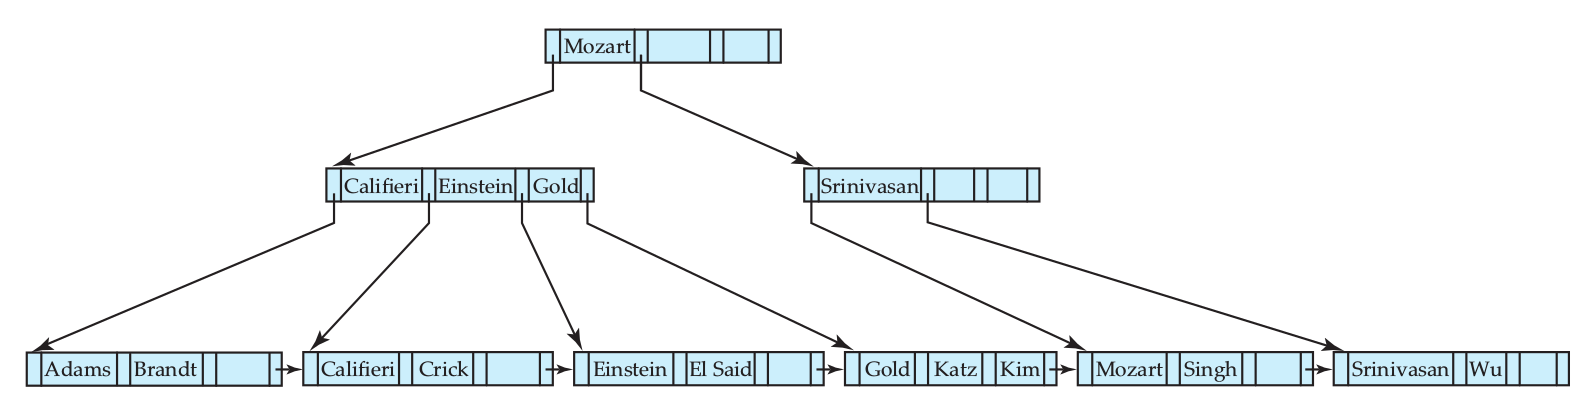
\includegraphics[width=0.9\textwidth]{images/b-tree-insert_adams.png}
\end{center}

\end{frame}


\begin{frame}
\frametitle{Exercise 4-6 Solution (2/2)}

\texttt{insert(Lamport)}

Follow the tree to find out where to insert Lamport.

It goes right of Gold/Katz/Kim, but the block is full.

As before, add Lamport conceptually, split the block into Gold/Katz and Kim/Lamport, and promote Kim.

Now the split blocks' parent (Califieri/Einstein/Gold/Kim) is oversized. Repeat the process.

Split into Califieri/Einstein and Gold/Kim, and promote Gold to the root, which becomes Gold/Mozart.

\begin{center}
  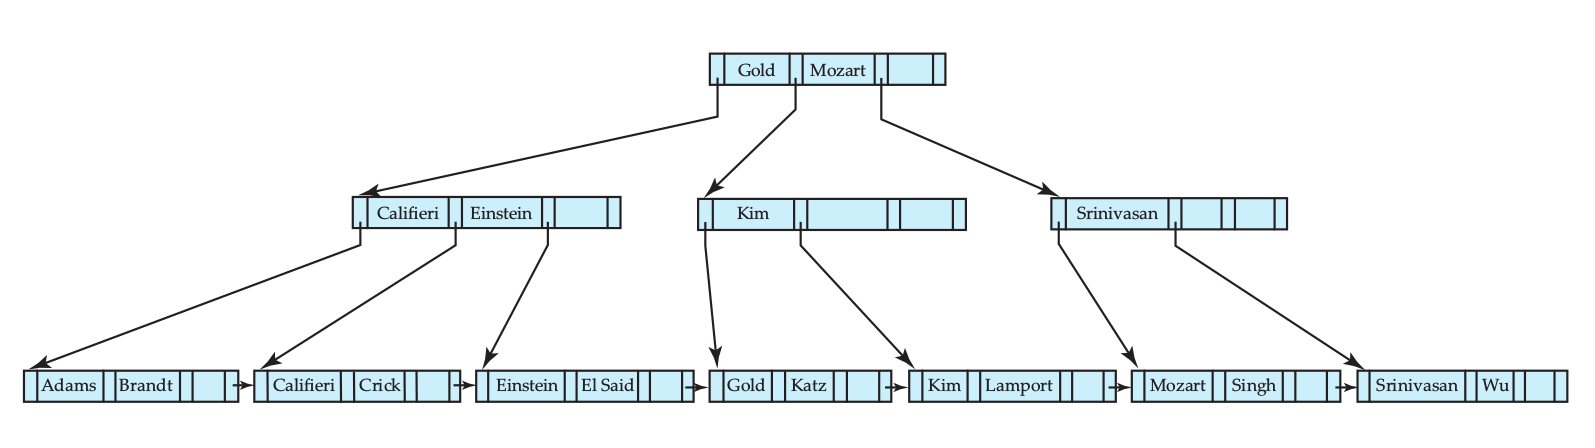
\includegraphics[width=0.9\textwidth]{images/b-tree-insert_lamport.png}
\end{center}

\end{frame}


\begin{frame}
\frametitle{Exercise 4-7}

Delete the following keys from the B+ tree below with degree $d$=2. Note that this tree does not have the value Lamport inserted, only Adam.

\texttt{Srinivasan}\\
\texttt{Singh}\\
\texttt{Wu}\\
\texttt{Gold}

\begin{center}
  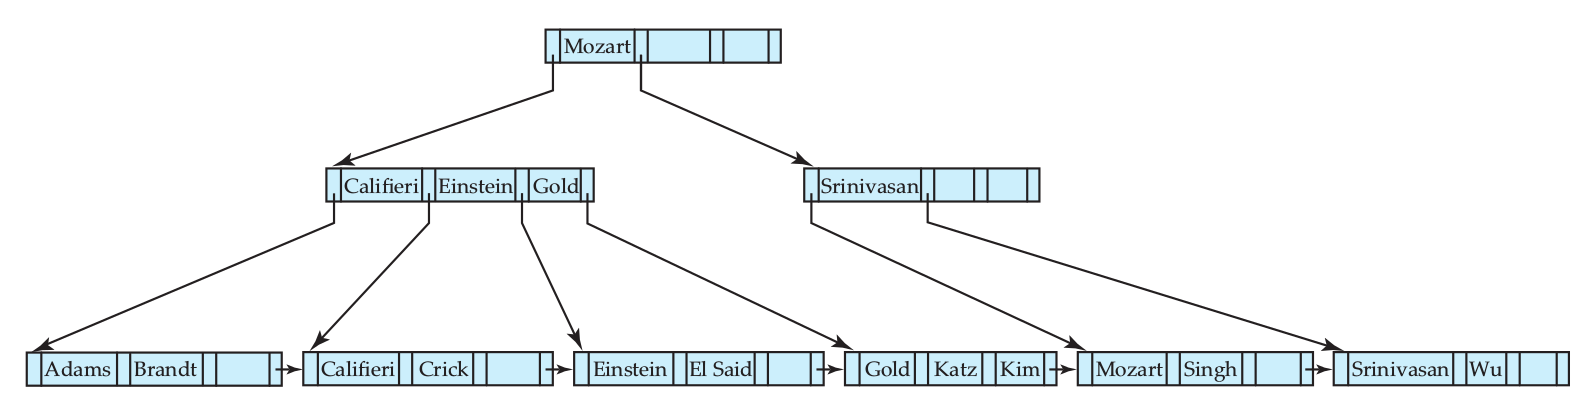
\includegraphics[width=0.9\textwidth]{images/b-tree-insert_adams.png}
\end{center}

\end{frame}


\begin{frame}
\frametitle{Exercise 4-7 Solution (1/3)}

\texttt{delete(Srinivasan)}

Remove Srinivasan from the Srinivasan/Wu node to leave Wu.

It is undersized and can merge with a sibling, so we merge Wu with Mozart/Singh to get Mozart/Singh/Wu.

The intermediate node Srinivasan only has one child, but cannot merge with its sibling Califieri/Einstein/Gold, so it steals a child of its sibling, Gold/Katz/Kim.

Update the keys of the intermediate nodes such that lookup still works.

\begin{center}
  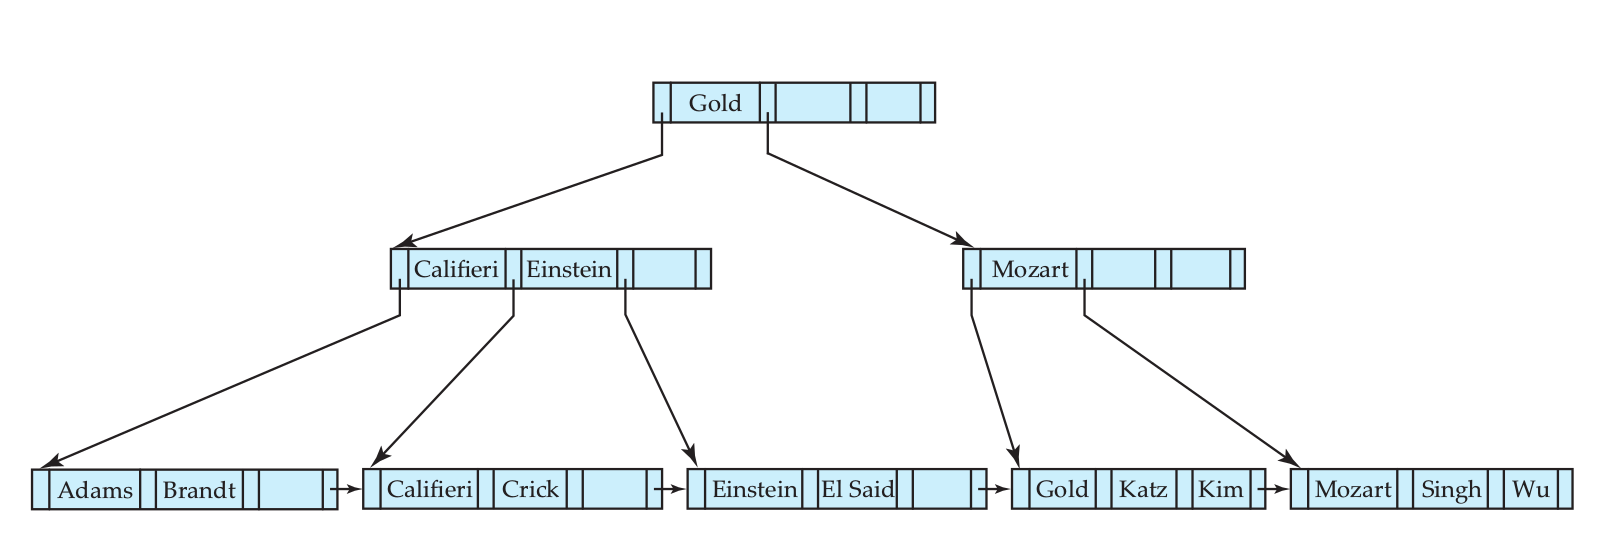
\includegraphics[width=0.9\textwidth]{images/b-tree-delete_srinivasan.png}
\end{center}

\end{frame}


\begin{frame}
\frametitle{Exercise 4-7 Solution (2/3)}

\texttt{delete(Singh)} \\
\texttt{delete(Wu)}

Removal of Singh and Wu are easy, since nothing complicated needs to happen.

The leaves after their removal violate no invariants and cannot be merged.


\begin{center}
  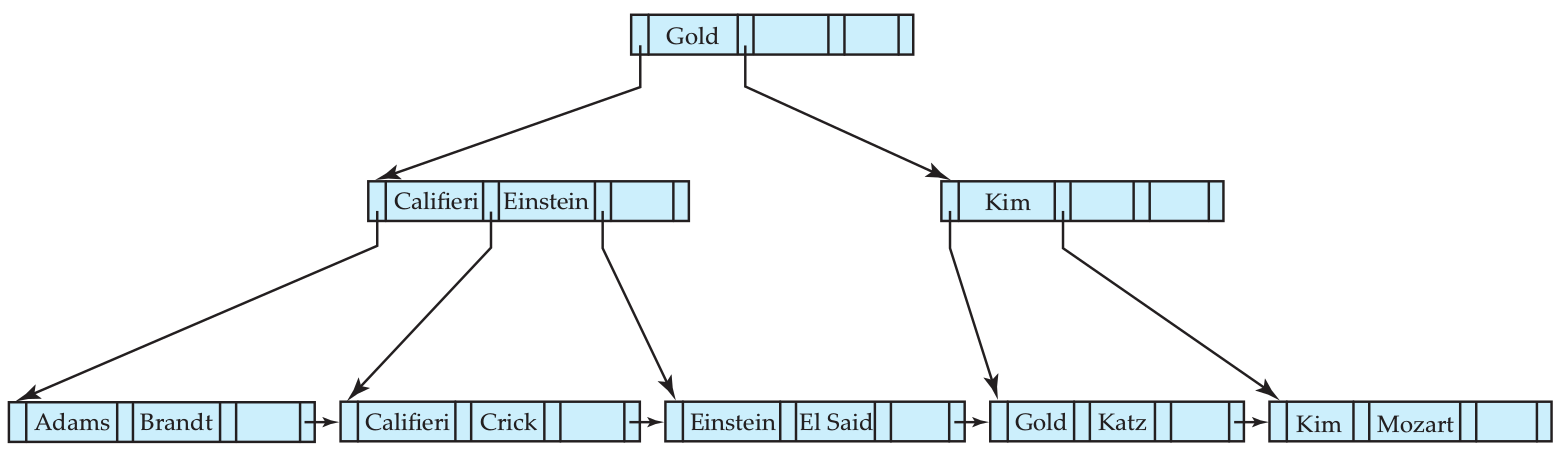
\includegraphics[width=0.9\textwidth]{images/b-tree-delete_singh_wu.png}
\end{center}

\end{frame}


\begin{frame}
\frametitle{Exercise 4-7 Solution (3/3)}

\texttt{delete(Gold)}

Removing Gold from Gold/Katz leaves a leaf that is undersized and can merge with Kim/Mozart to get Gold/Kim/Mozart.

The intermediate node Kim now is undersized, and is \textbf{able to merge} with its sibling, Califieri/Einstein, so it does.

We are left with one intermediate node, Califieri/Einstein/Kim, under the root node Gold.

The key replacement here merges keys from the root and the other intermediate node, leaving us with a new root, Califieri/Einstein/Gold.

An algorithm that leaves us with Califieri/Einstein/Katz would also be correct.

\begin{center}
  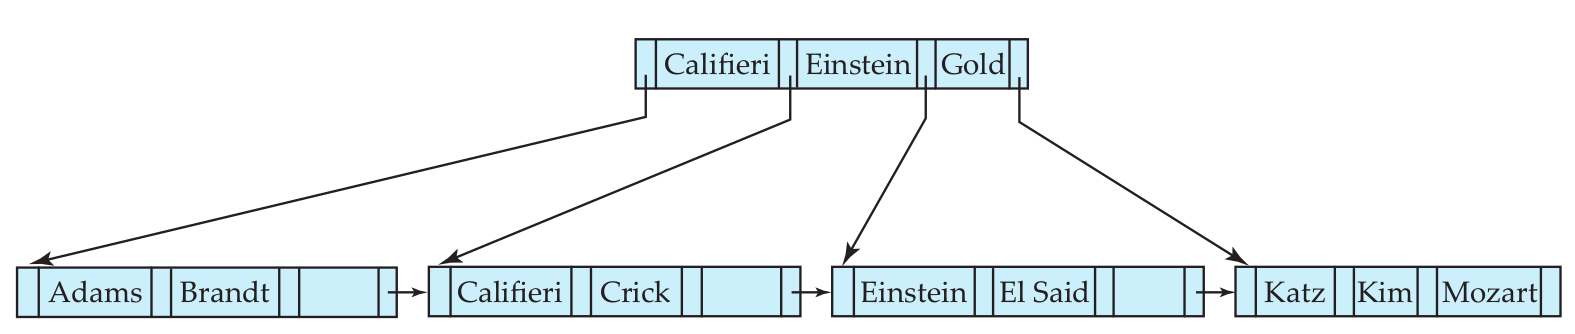
\includegraphics[width=0.9\textwidth]{images/b-tree-delete_gold.png}
\end{center}

\end{frame}


\begin{frame}
\frametitle{Resources}

The B+ tree example discussed in these slides are sourced from \texttt{Database System Concepts, Sixth Edition}, \textbf{starting on page 491}. In case you don't have the book, Professor Google is kind.

\end{frame}

\end{document}
